\chapter{Control Automático}
\section{Introducción}

El control es un área de la ingeniería y forma parte de la Ingeniería de
Control. Se centra en el control de los sistemas dinámicos mediante el principio
de la realimentación, para conseguir que las salidas de los mismos se acerquen
lo más posible a un comportamiento predefinido. Esta rama de la ingeniería tiene
como herramientas los métodos de la teoría de sistemas matemática.

Las bases de esta ingeniería se sentaron a mediados del Siglo XX a partir de la
cibernética. Sus principales aportaciones corresponden a Norbert Wiener, Rudolf
Kalman y David G. Luenberger.

La ingeniería de control es una ciencia interdisciplinar relacionada con muchos
otros campos, principalmente las matemáticas y la informática. Las aplicaciones
son de lo más variado: desde tecnología de fabricación, instrumentación médica,
Subestación eléctrica, ingeniería de procesos, robótica hasta economía y
sociología. Aplicaciones típicas son, por ejemplo, el piloto automático de
aviones y barcos y el ABS de los automóviles. En la biología se pueden encontrar
también sistemas de control realimentados, como por ejemplo el habla humana,
donde el oído recoge la propia voz para regularla.

El control de temperatura en una habitación es un ejemplo claro y típico de una
aplicación de ingeniería de control. El objetivo es mantener la temperatura de
una habitación en un valor deseado, aunque la apertura de puertas y ventanas y
la temperatura en el exterior hagan que la cantidad de calor que pierde la
habitación sean variables (perturbaciones externas). Para alcanzar el objetivo,
el sistema de calefacción debe modificarse para compensar esas perturbaciones.
Esto se hace a través del termostato, que mide la temperatura actual y la
temperatura deseada, y modifica la temperatura del agua del sistema de
calefacción para reducir la diferencia entre las dos temperaturas.
\begin{figure}
  \centering
    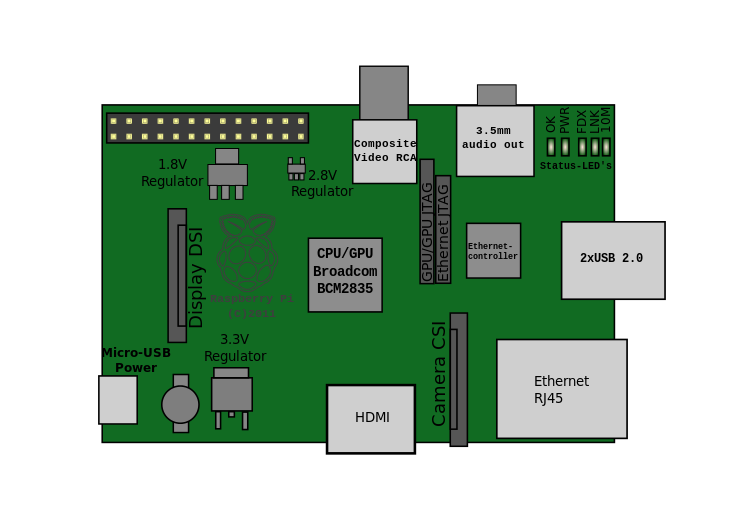
\includegraphics[width=0.5\textwidth]{raspi_pcb}
  \caption{Ubicación de los componentes de Raspberry Pi. \cite{raspberry_pi_wiki}}
  \label{fig:raspi_pcb}
\end{figure}

\begin{table}
\centering
  \begin{tabular}{r r r r}
\textbf{Pin} & \textbf{Descripción} & \textbf{Pin} & \textbf{Descripción} \\
\hline
1 & \texttt{3.3v} & 2 & \texttt{5v} \\
3 & \texttt{SDA0*} & 4 & \texttt{5v} \\
5 & \texttt{SCL0*} & 6 & \texttt{GND} \\
7 &  \texttt{GPIO\_GCLK} & 8 & \texttt{TXD0*} \\
9 &  \texttt{GND} & 10 & \texttt{RXD0*} \\
11 &  \texttt{GPIO\_GEN0} & 12 & \texttt{GPIO\_GEN1} \\
13 &  \texttt{GPIO\_GEN2} & 14 & \texttt{GND} \\
15 &  \texttt{GPIO\_GEN3} & 16 & \texttt{GPIO\_GEN4} \\
17 &  \texttt{3.3v} & 18 & \texttt{GPIO\_GEN5} \\
19 &  \texttt{SPI\_MOSI*} & 20 & \texttt{GND} \\
21 &  \texttt{SPI\_MISO*} & 22 & \texttt{GPIO\_GEN6} \\
23 &  \texttt{SPI\_SCLK*} & 24 & \texttt{SPI\_CEO\_N*} \\
25 &  \texttt{GND} & 26 & \texttt{SPI\_CE1\_N*} \\
  \end{tabular}
  \caption{Descripción de los pines de GPIO}
  \label{table:gpio_descr}
\end{table}

\section{Conclusiones}

blah blah.
